
\documentclass[12pt]{report} 

\usepackage[croatian]{babel} 
\usepackage{amssymb}
\usepackage{amsmath}
\usepackage{txfonts}
\usepackage{mathdots}
\usepackage{titlesec}
\usepackage{array}
\usepackage{lastpage}
\usepackage{etoolbox}
\usepackage{longtable, tabu}
\usepackage{color, colortbl}
\usepackage{adjustbox}
\usepackage{geometry}
\usepackage[classicReIm]{kpfonts}
\usepackage{hyperref}
\usepackage{fancyhdr}
\usepackage{graphicx}
\usepackage{hyperref}

\usepackage{float}
\usepackage{setspace}
\restylefloat{table}


\patchcmd{\chapter}{\thispagestyle{plain}}{\thispagestyle{fancy}}{}{}


\titleformat{\chapter}{\normalfont\huge\bfseries}{\thechapter.}{20pt}{\Huge}
\titlespacing{\chapter}{0pt}{0pt}{40pt}
\linespread{1.3}

\geometry{
	a4paper,
	left=1in,
	top=1in,
}

\hypersetup{ colorlinks, citecolor=black, filecolor=black, linkcolor=black,	urlcolor=black }


\newenvironment{packed_enum}{
	\begin{enumerate}
		\setlength{\itemsep}{0pt}
		\setlength{\parskip}{0pt}
		\setlength{\parsep}{0pt}
	}{\end{enumerate}}

\newenvironment{packed_item}{
	\begin{itemize}
		\setlength{\itemsep}{0pt}
		\setlength{\parskip}{0pt}
		\setlength{\parsep}{0pt}
	}{\end{itemize}}


\definecolor{LightBlue}{rgb}{0.9,0.9,1}
\definecolor{LightGreen}{rgb}{0.9,1,0.9}


%podesavanje headera i footera


\pagestyle{fancy}
\lhead{Oblikovanje programske potpore}
\rhead{Poliklinika za rehabilitaciju}
\lfoot{Flow}
\cfoot{stranica \thepage/\pageref{LastPage}}
\rfoot{\today}
\renewcommand{\headrulewidth}{0.2pt}
\renewcommand{\footrulewidth}{0.2pt}


\begin{document}
	

	\begin{titlepage}
		\begin{center}
			\vspace*{\stretch{1.0}}
			\LARGE Oblikovanje programske potpore\\
			\large Ak. god. 2019./2020.\\
			
			\vspace*{\stretch{3.0}}
			
			\huge Poliklinika za rehabilitaciju\\
			\Large Dokumentacija\\
			
			\vspace*{\stretch{12.0}}
			\normalsize
			Grupa: \textit{Flow}\\
			Voditelj: \textit{Marko Malkoč}\\
			
			
			\vspace*{\stretch{1.0}}
			Datum predaje: \textit{16.1.2020.}\\
	
			\vspace*{\stretch{4.0}}
			
			Nastavnik: \textit{Hrvoje Nuić}\\
		
		\end{center}

	
	\end{titlepage}

	
	\tableofcontents
	\chapter{Dnevnik promjena dokumentacije}
				
		
		\begin{longtabu} to \textwidth {|X[2, l]|X[13, l]|X[3, l]|X[3, l]|}
			\hline \multicolumn{1}{|l|}{\textbf{Rev.}}	& \multicolumn{1}{l|}{\textbf{Opis promjene/dodatka}} & \multicolumn{1}{|l|}{\textbf{Autori}} & \multicolumn{1}{l|}{\textbf{Datum}} \\[3pt] \hline
			\endfirsthead
			
			\hline \multicolumn{1}{|l|}{\textbf{Rev.}}	& \multicolumn{1}{l|}{\textbf{Opis promjene/dodatka}} & \multicolumn{1}{|l|}{\textbf{Autori}} & \multicolumn{1}{l|}{\textbf{Datum}} \\[3pt] \hline
			\endhead
			
			\hline 
			\endlastfoot
			
			0.1 & Napravljen predložak.	& Malkoč & 14.10.2019. 		\\[3pt] \hline 
			0.2	& Započeo nefunkcionalne zahtjeve, nefunkcionalne dijelove, opis arhitekture sustava & Juričić & 28.10.2019. 	\\[3pt] \hline 
			0.3 & Napisani dionici, aktori i njihovi opisi & Čižmešija & 28.10.2019. \\[3pt] \hline 
			0.4 & Dorađeni funkcionalni zahtjevi & Malkoč & 28.10.2019. \\[3pt] \hline 
			0.5 & Dodan prvi obrazac uporabe & Malkoč & 28.10.2019. \\[3pt] \hline 
			0.6 & Reorganizacija datoteka i uređeni funkcionalni zahtjevi & Malkoč & 02.11.2019. \\[3pt] \hline 
			0.7 & Dodan opis baze & Bakula & 03.11.2019. \\[3pt] \hline 
			0.8 & Dodani obrasci uporabe i reformatirani nefunkcionalni zahtjevi & Malkoč & 05.11.2019. \\[3pt] \hline 
			0.9 & Uređene tablice baze podataka & Bakula & 10.11.2019. \\[3pt] \hline 
			0.10 & Napisani dijagrami razreda & Ereš, Zanetti & 14.11.2019. \\[3pt] \hline
			0.11 & Ubačene slike obrazaca uporabe & Čižmešija & 15.11.2019. \\[3pt] \hline
			0.12 & Dodan opis projektnog zadatka & Omrčen & 15.11.2019. \\[3pt] \hline
			0.13 & Uređeno poglavlje Specifikacija programske potpore & Malkoč & 15.11.2019. \\[3pt] \hline
			0.14 & Dodan dijagram baza i ključevi & Bakula & 15.11.2019. \\[3pt] \hline
			0.15 & Dodani sekvencijski dijagrami i opis dijagrama razreda & Zanetti, Ereš & 15.11.2019. \\[3pt] \hline
			0.16 & Izmijenjen opis arhitekture sustava & Juričić & 15.11.2019. \\[3pt] \hline
			0.17 & Dnevnik sastanaka & Ereš & 15.11.2019. \\[3pt] \hline
			0.18 & Uređena tablica aktivnosti & Malkoč & 15.11.2019. \\[3pt] \hline
			0.19 & Dnevnik promjena dokumentacije & Zanetti & 15.11.2019. \\[3pt] \hline   
			\textbf{1.0} & Verzija samo s bitnim dijelovima za 1. ciklus & Malkoč & 15.11.2019. \\[3pt] \hline 
			
			
			
		\end{longtabu}
	

	\chapter{Opis projektnog zadatka Flow}
		
		\textbf{\textit{dio 1. revizije}}\\
		
		\textit{Na osnovi projektnog zadatka detaljno opisati korisničke zahtjeve. Što jasnije opisati cilj projektnog zadatka, razraditi problematiku zadatka, dodati nove aspekte problema i potencijalnih rješenja. Očekuje se minimalno 3, a poželjno 4-5 stranica opisa.	Teme koje treba dodatno razraditi u ovom poglavlju su:}
		\begin{packed_item}
			\item \textit{potencijalna korist ovog projekta}
			\item \textit{postojeća slična rješenja (istražiti i ukratko opisati razlike u odnosu na zadani zadatak). Dodajte slike koja predočavaju slična rješenja.}
			\item \textit{skup korisnika koji bi mogao biti zainteresiran za ostvareno rješenje.}
			\item \textit{mogućnost prilagodbe rješenja }
			\item \textit{opseg projektnog zadatka}
			\item \textit{moguće nadogradnje projektnog zadatka}
		\end{packed_item}
		
		\textit{Za pomoć pogledati reference navedene u poglavlju „Popis literature“, a po potrebi konzultirati sadržaj na internetu koji nudi dobre smjernice u tom pogledu.}
		\eject
		
		\section{Primjeri u LaTeXu}
		
		\textit{Ovo potpoglavlje izbrisati.}\\

		U nastavku se nalaze različiti primjeri kako koristiti osnovne funkcionalnosti LaTeXa koje su potrebne za izradu dokumentacije. Za dodatnu pomoć obratiti se asistentu na projektu ili potražiti upute na sljedećim web sjedištima:
		\begin{itemize}
			\item Upute za izradu diplomskog rada u LaTeXu - \url{https://www.fer.unizg.hr/_download/repository/LaTeX-upute.pdf}
			\item LaTeX projekt - \url{https://www.latex-project.org/help/}
			\item StackExchange za Tex - \url{https://tex.stackexchange.com/}\\
		
		\end{itemize} 	


		
		%Ovo poglavlje je potrebno prilikom predaje obrisati
		
		\underbar{podcrtani tekst}, 
		\textbf{podebljani tekst}, 
		\textit{nagnuti tekst}\\
		\normalsize primjer
		\large primjer
		\Large primjer
		\LARGE {primjer}
		\huge {primjer}
		\Huge primjer
		\normalsize
				
		\begin{packed_item}
			
			\item  primjer
			\item  primjer
			\item  primjer
			\item[] \begin{packed_enum}
				
				\item primjer
				\item primjer
			\end{packed_enum}
			
		\end{packed_item}
		
		\noindent primjer url-a: \url{https://www.fer.unizg.hr/predmet/opp/projekt}
		
		
		\begin{longtabu} to \textwidth {|X[8, l]|X[8, l]|X[16, l]|} %definicija sirine polja
			
			\hline \multicolumn{3}{|c|}{\textbf{naslov unutar tablice}}	 \\[3pt] \hline
			\endfirsthead
			
			\hline \multicolumn{3}{|c|}{\textbf{naslov unutar tablice}}	 \\[3pt] \hline
			\endhead
			
			\hline 
			\endlastfoot
			
			\rowcolor{LightGreen}IDKorisnik & INT	&  	Lorem ipsum dolor sit amet, consectetur adipiscing elit, sed do eiusmod  	\\ \hline
			korisnickoIme	& VARCHAR &   	\\ \hline 
			email & VARCHAR &   \\ \hline 
			ime & VARCHAR	&  		\\ \hline 
			\cellcolor{LightBlue} primjer	& VARCHAR &   	\\ \hline 
			
			
		\end{longtabu}
		

		\begin{table}[H]
			
			
			
			\begin{longtabu} to \textwidth {|X[8, l]|X[8, l]|X[16, l]|} %definicija sirine polja
				
				\hline 
				\endfirsthead
				
				\hline 
				\endhead
				
				\hline 
				\endlastfoot
				
				\rowcolor{LightGreen}IDKorisnik & INT	&  	Lorem ipsum dolor sit amet, consectetur adipiscing elit, sed do eiusmod  	\\ \hline
				korisnickoIme	& VARCHAR &   	\\ \hline 
				email & VARCHAR &   \\ \hline 
				ime & VARCHAR	&  		\\ \hline 
				\cellcolor{LightBlue} primjer	& VARCHAR &   	\\ \hline 
				
				
			\end{longtabu}
	
			\caption{\label{tab:referencatablica} Naslov ispod tablice.}
		\end{table}
		
		\begin{figure}[H]
			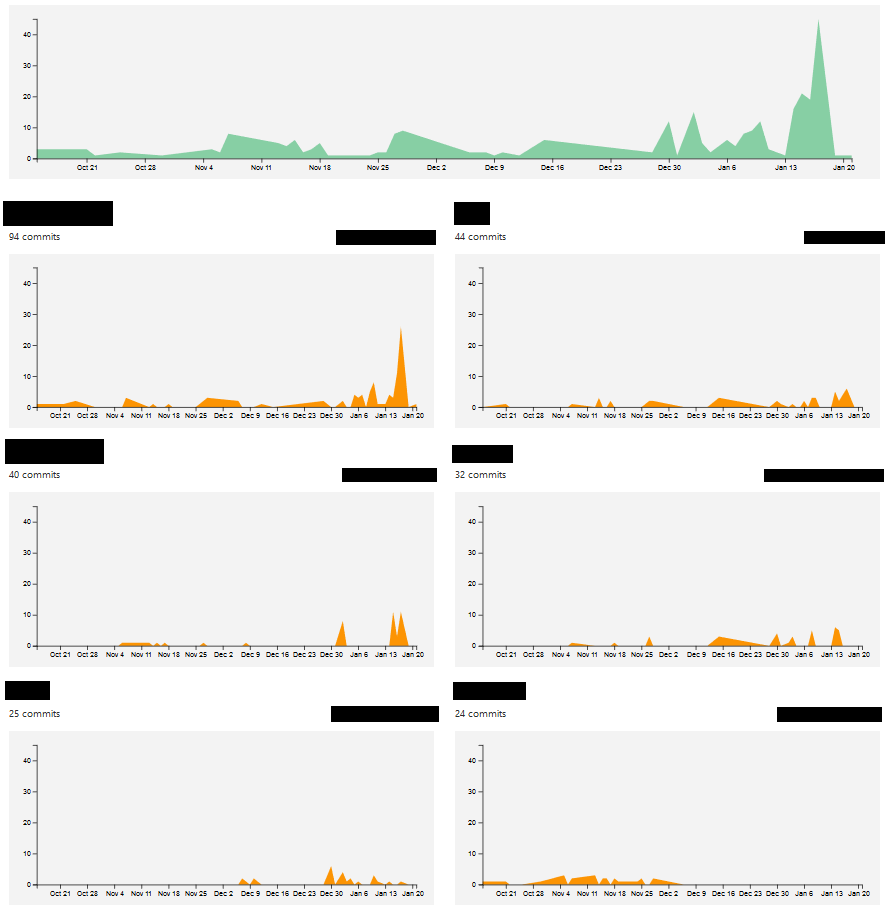
\includegraphics[scale=0.4]{slike/aktivnost.PNG}
			\centering
			\caption{Primjer slike s potpisom}
			\label{fig:promjene}
		\end{figure}
		
		\begin{figure}[H]
			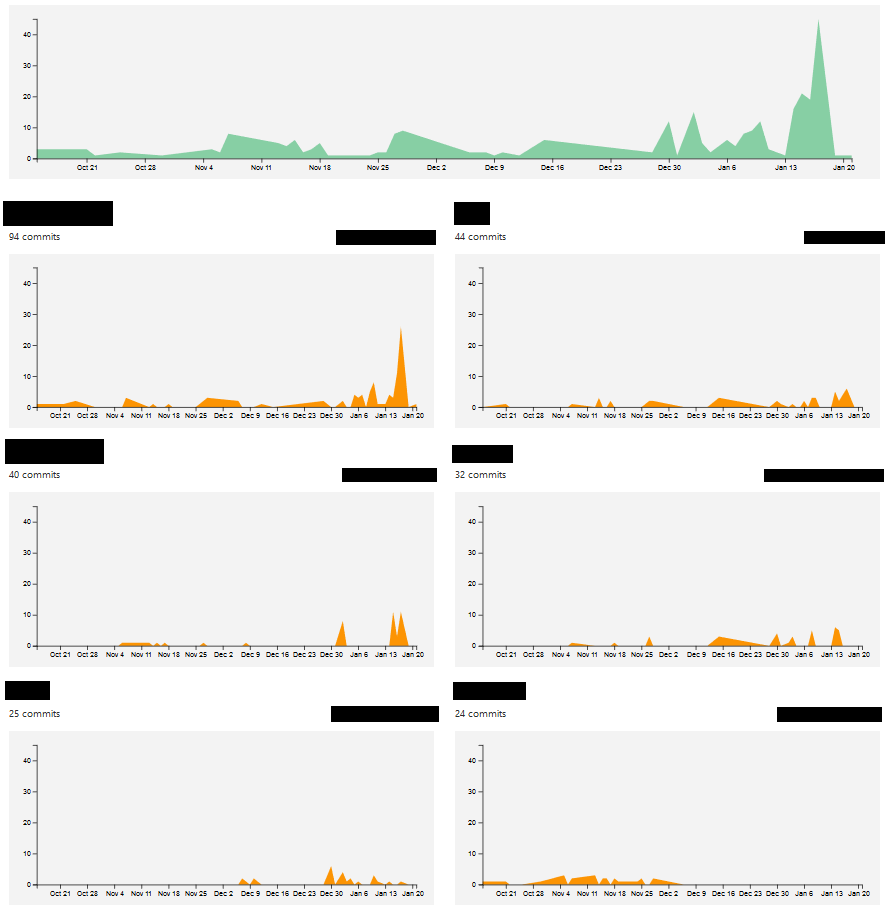
\includegraphics[width=\linewidth]{slike/aktivnost.PNG}
			\caption{Primjer slike s potpisom 2}
			\label{fig:promjene2}
		\end{figure}
		
		
		
		\eject
		
	
	\chapter{Specifikacija programske potpore}
		
	\section{Funkcionalni zahtjevi}
			
			\textit{ \textbf{Dionici} koji imaju interesa u ovom sustavu su svi \textbf{doktori, treneri i budući korisnici sustava},
			te dodatno \textbf{naručitelj projekta} (u ovom slučaju asistent tj. fakultet). Nositelji odgovornosti su \textbf{budući administratori sustava te razvojni tim}.}\\
				
			\textit{\textbf{Aktori} koji izravno koriste sustav su svi \textbf{doktori, treneri, klijenti i administratori}, dok sa sustavom neizravno komuniciraju \textbf{neregistrirani korisnici te baza podataka}.}\\
			
			
			\noindent \textbf{Dionici:}
			
			\begin{packed_enum}
				
				\item 1. Klijenti
				\item 2. Doktori			
				\item 3. Treneri
				\item 4. Razvojni tim (grupa Flow)
				\item 5. Naručitelj (asistent)
				\item 6. Administratori aplikacije
				
			\end{packed_enum}
			
			\noindent \textbf{Aktori i njihovi funkcionalni zahtjevi:}
			
			
			\begin{packed_enum}
				\item  \underbar{Administrator (inicijator) može:}
				
				\begin{packed_enum}
					
					\item potvrditi ili odbiti željenu ulogu neregistriranom korisniku

					\item dodavati proizvode i vježbe u kategorije
					
					\item uređivati i brisati
					\begin{packed_enum}
						
						\item kategorije
						\item proizvode
						\item vježbe
						
					\end{packed_enum}
				\end{packed_enum}
			
				\item  \underbar{Doktor (inicijator) može:}
				
				\begin{packed_enum}
					
					\item odgovarati na recenzije svojih klijenata
					\item prekinuti suradnju s klijentom
					\item definirati dijetu
					\begin{packed_enum}
						
						\item unositi sve potrebne parametre dijete
						\item dodati opis dijete
						
					\end{packed_enum}
				
					\item pregledati statistike klijenta po danu
					\item dodavati proizvode i vježbe u kategorije	
					
				\end{packed_enum}
			
				\item  \underbar{Trener (inicijator) može:}
				
				\begin{packed_enum}
					
					\item odgovarati na recenzije svojih klijenata
					\item prekinuti suradnju s klijentom
					\item definirati dnevne treninge
					\item pregledati statistike klijenta po danu
					\item dodavati proizvode i vježbe u kategorije
					
				\end{packed_enum}
			
				\item  \underbar{Klijent (inicijator) može:}
				
				\begin{packed_enum}
					
					\item tražiti i pregledavati profile svih dostupnih doktora i trenera
					\item ostaviti recenziju svom doktoru i treneru
					\item prekinuti suradnju sa svojim doktorom ili trenerom
					\item pregledati vlastite statistike po danu
					\item skenirati bar kod proizvoda koje planira konzumirati
					
				\end{packed_enum}
			
				\item  \underbar{Neregistrirani korisnik (inicijator) može:}
				
				\begin{packed_enum}
					
					\item registrirati se kao klijent
					\item poslati zahtjev za registraciju sa željenom ulogom
					
					\begin{packed_enum}
						
						\item trener
						\item doktor	
						
					\end{packed_enum}
					
				\end{packed_enum}
			
				\item  \underbar{Baza podataka (sudionik) može:}
				
				\begin{packed_enum}
					
					\item pohranjuje podatke o svim: 
					
					\begin{packed_enum}
						
						\item registriranim osobama
						\item recenzijama
						\item dijetama i proizvodima
						\item treninzima i vježbama
					
					\end{packed_enum}	
				
				\end{packed_enum}
			
			\end{packed_enum}
			
			\eject 
			
			
				
			\subsection{Obrasci uporabe}
				
				\subsubsection{Opis obrazaca uporabe}
					\textit{Funkcionalne zahtjeve razraditi u obliku obrazaca uporabe. Svaki obrazac je potrebno razraditi prema donjem predlošku. Ukoliko u nekom koraku može doći do odstupanja, potrebno je to odstupanje opisati i po mogućnosti ponuditi rješenje kojim bi se tijek obrasca vratio na osnovni tijek.}\\
					

					\noindent \underbar{\textbf{UC1 - Registracija klijenta}}
					\begin{packed_item}
	
						\item \textbf{Glavni sudionik:} Neregistrirani korisnik
						\item  \textbf{Cilj:} Stvoriti korisnički račun za pristup sustavu kao klijent
						\item  \textbf{Sudionici:} Baza podataka
						\item  \textbf{Preduvjet:} -
						\item  \textbf{Opis osnovnog tijeka:}
						
						\item[] \begin{packed_enum}
	
							\item Korisnik odabire opciju za registraciju klijenata
							\item Korisnik unosi potrebne podatke
							\item Korisnik potvrđuje podatke
							\item Sustav stvara novi korisnički račun i obavještava korisnika da je registracija uspješna
						\end{packed_enum}
						
						\item  \textbf{Opis mogućih odstupanja:}
						
						\item[] \begin{packed_item}
	
							\item[3.a] Unesesni podatci nisu ispravni
							\item[] \begin{packed_enum}
								
								\item Sustav obavještava korisnika o neuspjelom unosu i vraća ga na stranicu za registraciju
								\item Korisnik mijenja/dodaje potrebne podatke te završava unos ili odustaje od registracije
								
							\end{packed_enum}
							
						\end{packed_item}
					\end{packed_item}
				
					\noindent \underbar{\textbf{UC2 - Registracija zaposlenika}}
					\begin{packed_item}
						
						\item \textbf{Glavni sudionik:} Neregistrirani korisnik
						\item  \textbf{Cilj:} Stvoriti korisnički račun za pristup sustavu kao zaposlenik
						\item  \textbf{Sudionici:} Baza podataka
						\item  \textbf{Preduvjet:} -
						\item  \textbf{Opis osnovnog tijeka:}
						
						\item[] \begin{packed_enum}
							
							\item Korisnik odabire opciju za registraciju zaposlenika
							\item Korisnik unosi potrebne podatke
							\item Korisnik potvrđuje podatke
							\item Administrator potvrđuje zahtjev za registracijom
							\item Sustav stvara novi korisnički račun
						\end{packed_enum}
						
						\item  \textbf{Opis mogućih odstupanja:}
						
						\item[] \begin{packed_item}
							
							\item[3.a] Uneseni podatci nisu ispravni 
							\item[] \begin{packed_enum}
								
								\item Sustav obavještava korisnika o neuspjelom unosu i vraća ga na stranicu za registraciju
								\item Korisnik mijenja/dodaje potrebne podatke te završava unos ili odustaje od registracije
								
							\end{packed_enum}
						
							\item[4.a] Administrator odbija zahtjev
							\item [] \begin{packed_enum}
								
								\item Korisnik ne dobiva pristup sustavu
							
							\end{packed_enum}
						\end{packed_item}
					\end{packed_item}
				
					\noindent \underbar{\textbf{UC3 - Prijava u sustav}}
					\begin{packed_item}
						
						\item \textbf{Glavni sudionik:} Neprijavljeni korisnik
						\item  \textbf{Cilj:} Dobiti pristup korisničkom sučelju
						\item  \textbf{Sudionici:} Baza podataka
						\item  \textbf{Preduvjet:} Korisnik je registriran
						\item  \textbf{Opis osnovnog tijeka:}
						
						\item[] \begin{packed_enum}
							
							\item Korisnik unosi podatke potrebne za prijavu
							\item Korisnik potvrđuje unos
							\item Sustav prijavljuje korisnika i prikazuje korisničko sučelje
						\end{packed_enum}
						
						\item  \textbf{Opis mogućih odstupanja:}
						
						\item[] \begin{packed_item}
							
							\item[2.a] Uneseni podatci nisu ispravni
							\item[] \begin{packed_enum}
								
								\item Sustav obavještava korisnika o neuspjeloj prijavi i vraća ga na stranicu za prijavu
								
							\end{packed_enum}
						
							\item[3.a] Administrator nije još potvrdio korisnikov zahtjev za registraciju
							\item[] \begin{packed_enum}
								
								\item Sustav obavještava korisnika da njegov zahtjev još nije prihvaćen
								
							\end{packed_enum}
							
						\end{packed_item}
					\end{packed_item}
				
					\noindent \underbar{\textbf{UC4 - Potvrda zahtjeva neregistriranog korisnika}}
					\begin{packed_item}
						
						\item \textbf{Glavni sudionik:} Administrator
						\item  \textbf{Cilj:}  Potvrditi zahtjev neregistriranog korisnika
						\item  \textbf{Sudionici:} Baza podataka
						\item  \textbf{Preduvjet:} Korisnik je prijavljen
						\item  \textbf{Opis osnovnog tijeka:}
						
						\item[] \begin{packed_enum}
							
							\item Korisnik odabire prikaz zahtjeva za registraciju
							\item Korisnik potvrđuje željeni zahtjev
							\item Sustav stvara novi korisnički račun za osobu koja je poslala zahtjev
							
						\end{packed_enum}
						
						\item  \textbf{Opis mogućih odstupanja:}
						
						\item[] \begin{packed_item}
							
							\item[2.a] Zahtjev nije valjan
							\item[] \begin{packed_enum}
								
								\item Korisnik odbija zahtjev
								\item Sustav briše odbijeni zahtjev
								\item Sustav ponovo prikazuje zahtjeve za registracijom
								
							\end{packed_enum}
							
						\end{packed_item}
						
					\end{packed_item}
				
				
					\noindent \underbar{\textbf{UC5 - Slanje zahtjeva za suradnju}}
					\begin{packed_item}
						
						\item \textbf{Glavni sudionik:} Klijent
						\item  \textbf{Cilj:} Započeti suradnju sa željenim zaposlenikom
						\item  \textbf{Sudionici:} Baza podataka
						\item  \textbf{Preduvjet:} Korisnik je prijavljen
						\item  \textbf{Opis osnovnog tijeka:}
						
						\item[] \begin{packed_enum}
							
							\item Korisnik odabire pregled zaposlenika
							\item Korisnik odabire opciju za slanje zahtjeva željenom zaposleniku
							\item Zaposlenik kojem je slan zahtjev potvrđuje korisnika
							\item Korisnik i zaposlenik sada su u suradnji i sustav pohranjuje promjene u bazu podataka
							
						\end{packed_enum}
					
						\item	\textbf{Opis mogućih odstupanja:}
						
						\item[] \begin{packed_enum}
							
							\item[3.a] Zaposlenik odbija zahtjev
							\item[] \begin{packed_enum}
								
								\item Sustav obavještava korisnika da je njegov zahtjev odbijen
								
							\end{packed_enum}
						
						\end{packed_enum}
						
					\end{packed_item}
				
					\noindent \underbar{\textbf{UC6 - Potvrda zahtjeva za suradnju}}
					\begin{packed_item}
						
						\item \textbf{Glavni sudionik:} Doktor, trener
						\item  \textbf{Cilj:} Potvrditi zahtjev za suradnju koji je poslao klijent
						\item  \textbf{Sudionici:} Baza podataka
						\item  \textbf{Preduvjet:} Korisnik je prijavljen
						\item  \textbf{Opis osnovnog tijeka:}
						
						\item[] \begin{packed_enum}
							
							\item Korisnik odabire pregled zahtjeva za suradnju
							\item Korisnik potvrđuje željeni zahtjev
							\item Korisnik i klijent sada su u suradnji i sustav pohranjuje promjene u bazu podataka
							
						\end{packed_enum}
						
						\item  \textbf{Opis mogućih odstupanja:}
						
						\item[] \begin{packed_item}
							
							\item[2.a] Zahtjev nije valjan
							\item[] \begin{packed_enum}
								
								\item Korisnik odbija zahtjev
								\item Sustav javlja klijentu da je njegov zahtjev odbijen
								\item Sustav ponovno prikazuje pregled zahtjeva za suradnjom
								
							\end{packed_enum}
							
						\end{packed_item}	
						
					\end{packed_item}
				
					\noindent \underbar{\textbf{UC7 - Prekid suradnje}}
					\begin{packed_item}
						
						\item \textbf{Glavni sudionik:} Klijent, doktor, trener
						\item  \textbf{Cilj:} Prekinuti suradnju s osobom
						\item  \textbf{Sudionici:} Baza podataka
						\item  \textbf{Preduvjet:} Korisnik mora biti prijavljen i u suradnji s barem jednom osobom
						\item  \textbf{Opis osnovnog tijeka:}
						
						\item[] \begin{packed_enum}
							
							\item Korisnik odabire pregled svojih suradnika
							\item Korisnik odabire opciju za prekid suradnje s željenom osobom
							\item Korisnik i odabrana osoba više nisu u suradnji i sustav pohranjuje promjene u bazu podataka
							
						\end{packed_enum}
						
					\end{packed_item}
				
					\noindent \underbar{\textbf{UC8 - Ocjenjivanje zaposlenika}}
					\begin{packed_item}
						
						\item \textbf{Glavni sudionik:} Klijent
						\item  \textbf{Cilj:} Napisati recenziju zaposlenika s kojim je klijent u suradnji
						\item  \textbf{Sudionici:} Baza podataka
						\item  \textbf{Preduvjet:} Korisnik je prijavljen i u suradnji je s barem jednom osobom
						\item  \textbf{Opis osnovnog tijeka:}
						
						\item[] \begin{packed_enum}
							
							\item Korisnik odabire prikaz osoba s kojima je u suradnji
							\item Korisnik odabire kojeg zaposlenika želi ocijeniti
							\item Korisnik izabire ocjenu i piše komentar
							\item Korisnik potvrđuje unos
							\item Sustav pohranjuje recenziju u bazu podataka i ažurira prosječnu ocjenu zaposlenika
							
						\end{packed_enum}
					
						\item  \textbf{Opis mogućih odstupanja:}
						
						\item[] \begin{packed_item}
							
							\item[4.a] Nisu uneseni svi potrebni podatci
							\item[] \begin{packed_enum}
								
								\item Sustav obavještava korisnika da treba ispuniti sve potrebne podatke i vraća ga na stranicu za pisanje recenzije
								
							\end{packed_enum}
							
						\end{packed_item}
						
						
					\end{packed_item}
			
					\noindent \underbar{\textbf{UC9 - Odgovor na vlastitu recenziju}}
					\begin{packed_item}
						
						\item \textbf{Glavni sudionik:} Doktor, trener
						\item  \textbf{Cilj:} Odgovoriti na klijentovu recenziju
						\item  \textbf{Sudionici:} Baza podataka
						\item  \textbf{Preduvjet:} Korisnik je prijavljen i barem jedan klijent je napisao recenziju za njega
						\item  \textbf{Opis osnovnog tijeka:}
						
						\item[] \begin{packed_enum}
							
							\item Korisnik odabire pregled svojih recenzija
							\item Korisnik odabire opciju za odgovoriti na željenu recenziju
							\item Korisnik unosi potrebne podatke
							\item Korisnik potvrđuje unos
							\item Sustav pohranjuje odgovor u bazu podataka
							
						\end{packed_enum}
					
						\item  \textbf{Opis mogućih odstupanja:}
						
						\item[] \begin{packed_item}
							
							\item[4.a] Nisu uneseni svi potrebni podatci
							\item[] \begin{packed_enum}
								
								\item Sustav obavještava korisnika da treba ispuniti sve potrebne podatke i vraća ga na stranicu za odgovor na recenziju
								
							\end{packed_enum}
							
						\end{packed_item}
						
					\end{packed_item}
				
			
					\noindent \underbar{\textbf{UC10 - Definiranje dijete}}
					\begin{packed_item}
						
						\item \textbf{Glavni sudionik:} Doktor
						\item  \textbf{Cilj:} Definitrati dijetu svome klijentu
						\item  \textbf{Sudionici:} Baza podataka
						\item  \textbf{Preduvjet:} Korisnik je prijavljen i u suradnji je s barem jednim klijentom
						\item  \textbf{Opis osnovnog tijeka:}
						
						\item[] \begin{packed_enum}
							
							\item Korisnik odabire pregled svojih klijenata
							\item Korisnik odabire opciju za definiranje dijete željenom klijentu
							\item Korisnik unosi potrebne podatke
							\item Korisnik potvrđuje unos
							\item Sustav pohranjuje promjene u bazu podataka
							
						\end{packed_enum}
					
						\item  \textbf{Opis mogućih odstupanja:}
						
						\item[] \begin{packed_item}
							
							\item[4.a] Nisu uneseni svi potrebni podatci
							\item[] \begin{packed_enum}
								
								\item Sustav obavještava korisnika da treba ispuniti sve potrebne podatke i vraća ga na stranicu za definiranje dijete
								
							\end{packed_enum}
							
						\end{packed_item}
						
					\end{packed_item}
				
					\noindent \underbar{\textbf{UC11 - Definiranje treninga}}
					\begin{packed_item}
						
						\item \textbf{Glavni sudionik:} Trener
						\item  \textbf{Cilj:} Definirati trening svome klijentu
						\item  \textbf{Sudionici:} Baza podataka
						\item  \textbf{Preduvjet:} Korisnik je prijavljen i u suradnji s barem jednim klijentom
						\item  \textbf{Opis osnovnog tijeka:}
						
						\item[] \begin{packed_enum}
							
							\item Korisnik odabire prikaz svojih klijenata
							\item Korisnik odabire opciju za definiranje treninga željenom klijentu
							\item Korisnik unosi potrebne podatke
							\item Korisnik potvrđuje unos
							\item Sustav pohranjuje promjene u bazu podataka
							
						\end{packed_enum}
						
						\item  \textbf{Opis mogućih odstupanja:}
						
						\item[] \begin{packed_item}
							
							\item[4.a] Nisu uneseni svi potrebni podatci
							\item[] \begin{packed_enum}
								
								\item Sustav obavještava korisnika da treba ispuniti sve potrebne podatke i vraća ga na stranicu za definiranje treninga
								
							\end{packed_enum}
							
						\end{packed_item}
						
					\end{packed_item}
			
					\noindent \underbar{\textbf{UC12 - Pregled statistike klijenta}}
					\begin{packed_item}
						
						\item \textbf{Glavni sudionik:} Doktor, trener
						\item  \textbf{Cilj:} Pregledati statustiku klijenta po danu
						\item  \textbf{Sudionici:} Baza podataka
						\item  \textbf{Preduvjet:} Korisnik je prijavljen i u suradnji je s barem jednim klijentom
						\item  \textbf{Opis osnovnog tijeka:}
						
						\item[] \begin{packed_enum}
							
							\item Korisnik odabire pregled svojih klijenata
							\item Korisnik odabire opciju za pregled statistike željenog klijenta
							\item Korisnik odabire za koji dan se prikazuje statistika
							\item Sustav prikazuje statistiku klijenta za taj dan
							
						\end{packed_enum}
					
						\item  \textbf{Opis mogućih odstupanja:}
						
						\item[] \begin{packed_item}
							
							\item[4.a] Klijent nema upisanih podataka 
							\item[] \begin{packed_enum}
								
								\item Sustav obavještava da klijent nema upisanih podataka za taj dan i nudi opciju za povratak
								
							\end{packed_enum}
							
						\end{packed_item}	
						
					\end{packed_item}
			
					\noindent \underbar{\textbf{UC13 - Pregled svoje statistike}}
					\begin{packed_item}
						
						\item \textbf{Glavni sudionik:} Klijent
						\item  \textbf{Cilj:} Pregledati svoju statistiku po danu
						\item  \textbf{Sudionici:} Baza podataka
						\item  \textbf{Preduvjet:} Korisnik je prijavljen
						\item  \textbf{Opis osnovnog tijeka:}
						
						\item[] \begin{packed_enum}
							
							\item Korisnik odabire opciju za prikaz statistike
							\item Korisnik odabire za koji dan se prikazuje statistika
							\item Sustav prikazuje statistiku za taj dan
							
						\end{packed_enum}
					
						\item  \textbf{Opis mogućih odstupanja:}
						
						\item[] \begin{packed_item}
							
							\item[3.a] Klijent nema upisanih podataka 
							\item[] \begin{packed_enum}
								
								\item Sustav obavještava da nema upisanih podataka i nudi opciju za povratak
								
							\end{packed_enum}
							
						\end{packed_item}
						
					\end{packed_item}
			
					\noindent \underbar{\textbf{UC14 - Dodavanje proizvoda u kategoriju}}
					\begin{packed_item}
						
						\item \textbf{Glavni sudionik:} Doktor, trener, administrator
						\item  \textbf{Cilj:} Dodati proizvod u željenu kategoriju
						\item  \textbf{Sudionici:} Baza podataka
						\item  \textbf{Preduvjet:} Korisnik je prijavljen
						\item  \textbf{Opis osnovnog tijeka:}
						
						\item[] \begin{packed_enum}
							
							\item Korisnik odabire prikaz kategorija proizvoda
							\item Korisnik odabire željenu kategoriju
							\item Korisnik dodaje željene proizvode u kategoriju
							\item Sustav pohranjuje promjene bazu podataka
							
						\end{packed_enum}
					
					\end{packed_item}
			
					\noindent \underbar{\textbf{UC15 - Dodavanje vježbe u kategoriju}}
					\begin{packed_item}
						
						\item \textbf{Glavni sudionik:} Doktor, trener, administrator
						\item  \textbf{Cilj:} Dodati vježbu u željenu kategoriju
						\item  \textbf{Sudionici:} Baza podataka
						\item  \textbf{Preduvjet:} Korisnik je prijavljen
						\item  \textbf{Opis osnovnog tijeka:}
						
						\item[] \begin{packed_enum}
							
							\item Korisnik odabire prikaz kategorija vježbi
							\item Korisnik odabire željenu kategoriju
							\item Korisnik dodaje željene vježbe u kategoriju
							\item Sustav pohranjuje promjene u bazu podataka
							
						\end{packed_enum}
						
					\end{packed_item}
			
					\noindent \underbar{\textbf{UC16 - Stvaranje kategorije}}
					\begin{packed_item}
						
						\item \textbf{Glavni sudionik:} Administrator
						\item  \textbf{Cilj:} Stvoriti novu kategoriju
						\item  \textbf{Sudionici:} Baza podataka
						\item  \textbf{Preduvjet:} Korisnik je prijavljen
						\item  \textbf{Opis osnovnog tijeka:}
						
						\item[] \begin{packed_enum}
							
							\item Korisnik odabire prikaz kategorija
							\item Korisnik odabire opciju za kreiranje nove kategorije
							\item Korisnik unosi potrebne podatke o kategoriji i njen sadržaj
							\item Korisnik potvrđuje unos
							\item Sustav pohranjuje novu kategoriju u bazu podataka
							
						\end{packed_enum}
						
						\item  \textbf{Opis mogućih odstupanja:}
						
						\item[] \begin{packed_item}
							
							\item[4.a] Nisu uneseni svi potrebni podatci
							\item[] \begin{packed_enum}
								
								\item Sustav obavještava korisnika da treba unijeti sve potrebne podatke i vraća ga na stranicu za stvaranje kategorije
								
							\end{packed_enum}
							
						\end{packed_item}
						
					\end{packed_item}
			
					\noindent \underbar{\textbf{UC17 - Uređivanje kategorija}}
					\begin{packed_item}
						
						\item \textbf{Glavni sudionik:} Administrator
						\item  \textbf{Cilj:} Izmijenti sadržaj kategorije i podatke o kategoriji
						\item  \textbf{Sudionici:} Baza podataka
						\item  \textbf{Preduvjet:} Korisnik je prijavljen i postoji barem jedna kategorija
						\item  \textbf{Opis osnovnog tijeka:}
						
						\item[] \begin{packed_enum}
							
							\item Korisnik odabire prikaz kategorija
							\item Korisnik odabire kategoriju koju želi izmijeniti
							\item Korisnik mijenja podatke o kategoriji i njen sadržaj
							\item Korisnik potvrđuje izmjenu
							\item Promjene se pohranjuju u bazu podataka
							
						\end{packed_enum}
						
						\item  \textbf{Opis mogućih odstupanja:}
						
						\item[] \begin{packed_item}
							
							\item[4.a] Izmijenjeni podatci nisu ispravni 
							\item[] \begin{packed_enum}
								
								\item Sustav obavještava korisnika da mora unijeti ispravne podatke i vraća ga na stranicu za uređivanje kategorije
								
							\end{packed_enum}
							
						\end{packed_item}
						
					\end{packed_item}
				
				
					\noindent \underbar{\textbf{UC18 - Brisanje kategorije}}
					\begin{packed_item}
						
						\item \textbf{Glavni sudionik:} Administrator
						\item  \textbf{Cilj:} Obrisati kategoriju
						\item  \textbf{Sudionici:} Baza podataka
						\item  \textbf{Preduvjet:} Korisnik je prijavljen i postoji barem jedna kategorija
						\item  \textbf{Opis osnovnog tijeka:}
						
						\item[] \begin{packed_enum}
							
							\item Korisnik odabire prikaz kategorija
							\item Korisnik odabire opciju za brisanje željene kategorije
							\item Sustav briše kategoriju i pohranjuje promjene u bazu podataka
							
						\end{packed_enum}
						
					\end{packed_item}
				
					\noindent \underbar{\textbf{UC19 - Dodavanje proizvoda}}
					\begin{packed_item}
						
						\item \textbf{Glavni sudionik:} Administrator
						\item  \textbf{Cilj:} Dodati novi proizvod u sustav
						\item  \textbf{Sudionici:} Baza podataka
						\item  \textbf{Preduvjet:} Korisnik je prijavljen
						\item  \textbf{Opis osnovnog tijeka:}
						
						\item[] \begin{packed_enum}
							
							\item Korisnik odabire prikaz proizvoda
							\item Korisnik odabire opciju za dodavanje novog proizvoda
							\item Korisnik unosi sve potrebne podatke
							\item Korisnik potvrđuje unos
							\item Sustav dodaje proizvod i pohranjuje ga u bazu podataka
							
						\end{packed_enum}
						
						\item  \textbf{Opis mogućih odstupanja:}
						
						\item[] \begin{packed_item}
							
							\item[4.a] Nisu uneseni svi potrebni podatci
							\item[] \begin{packed_enum}
								
								\item Sustav obavještava korisnika da treba unijeti sve potrebne podatke i vraća ga na stranicu za dodavanje proizvoda
								
							\end{packed_enum}
							
						\end{packed_item}	
							
					\end{packed_item}
				
					\noindent \underbar{\textbf{UC20 - Uređivanje proizvoda}}
					\begin{packed_item}
						
						\item \textbf{Glavni sudionik:} Administrator
						\item  \textbf{Cilj:} Izmijeniti podatke o željenom proizvodu
						\item  \textbf{Sudionici:} Baza podataka
						\item  \textbf{Preduvjet:} Korisnik je prijavljen i dodan je barem jedan proizvod
						\item  \textbf{Opis osnovnog tijeka:}
						
						\item[] \begin{packed_enum}
							
							\item Korisnik odabire prikaz proizvoda
							\item Korisnik odabire opciju za uređivanje željenog proizvoda
							\item Korisnik mijenja podatke o proizvodu
							\item Korisnik potvrđuje izmjenu
							\item Sustav pohranjuje promjenu u bazu podataka
							
						\end{packed_enum}
						
						\item  \textbf{Opis mogućih odstupanja:}
						
						\item[] \begin{packed_item}
							
							\item[4.a] Izmijenjeni podatci nisu ispravni 
							\item[] \begin{packed_enum}
								
								\item Sustav obavještava korisnika da mora unijeti ispravne podatke i vraća ga na stranicu za uređivanje proizvoda
								
							\end{packed_enum}
							
						\end{packed_item}	
						
					\end{packed_item}
				
					\noindent \underbar{\textbf{UC21 - Brisanje proizvoda}}
					\begin{packed_item}
						
						\item \textbf{Glavni sudionik:} Administrator
						\item  \textbf{Cilj:} Obrisati proizvod
						\item  \textbf{Sudionici:} Baza podataka
						\item  \textbf{Preduvjet:} Korisnik je prijavljen i dodan je barem jedan proizvod
						\item  \textbf{Opis osnovnog tijeka:}
						
						\item[] \begin{packed_enum}
							
							\item Korisnik odabire prikaz proizvoda
							\item Korisnik odabire opciju za brisanje željenog proizvoda
							\item Sustav briše proizvod i pohranjuje promjene u bazu podataka
							
						\end{packed_enum}
							
						
					\end{packed_item}
				
					\noindent \underbar{\textbf{UC22 - Dodavanje vježbe}}
					\begin{packed_item}
						
						\item \textbf{Glavni sudionik:} Administrator
						\item  \textbf{Cilj:} Dodati novu vježbu u sustav
						\item  \textbf{Sudionici:} Baza podataka
						\item  \textbf{Preduvjet:} Korisnik je prijavljen
						\item  \textbf{Opis osnovnog tijeka:}
						
						\item[] \begin{packed_enum}
							
							\item Korisnik odabire prikaz vježbi
							\item Korisnik odabire opciju za dodavanje vježbe
							\item Korisnik unosi sve potrebne podatke
							\item Korisnik potvrđuje unos
							\item Sustav stvara novu vježbu i pohranjuje izmijene u bazu podataka
							
						\end{packed_enum}
						
						\item  \textbf{Opis mogućih odstupanja:}
						
						\item[] \begin{packed_item}
							
							\item[4.a] Nisu uneseni svi potrebni podatci
							\item[] \begin{packed_enum}
								
								\item Sustav obavještava korisnika da treba unijeti sve potrebne podatke i vraća ga na stranicu za dodavanje vježbe
								
							\end{packed_enum}
							
						\end{packed_item}	
						
					\end{packed_item}
					
					\noindent \underbar{\textbf{UC23 - Uređivanje vježbe}}
					\begin{packed_item}
						
						\item \textbf{Glavni sudionik:} Administrator
						\item  \textbf{Cilj:} Izmijeniti podatke o željenoj vježbi
						\item  \textbf{Sudionici:} Baza podataka
						\item  \textbf{Preduvjet:} Korisnik je prijavljen i dodana je barem jedna vježba
						\item  \textbf{Opis osnovnog tijeka:}
						
						\item[] \begin{packed_enum}
							
							\item Korisnik odabire prikaz vježbi
							\item Korisnik odabire opciju za uređivanje željenog proizvoda
							\item Korisnik mijenja podatke o vježbi
							\item Korisnik potvrđuje izmjenu
							\item Sustav pohranjuje promjenu u bazu podataka
							
						\end{packed_enum}
						
						\item  \textbf{Opis mogućih odstupanja:}
						
						\item[] \begin{packed_item}
							
							\item[4.a] Izmijenjeni podatci nisu ispravni 
							\item[] \begin{packed_enum}
								
								\item Sustav obavještava korisnika da mora unijeti ispravne podatke i vraća ga na stranicu za uređivanje vježbe
								
							\end{packed_enum}
							
						\end{packed_item}	
						
					\end{packed_item}
					
					\noindent \underbar{\textbf{UC24 - Brisanje vježbe}}
					\begin{packed_item}
						
						\item \textbf{Glavni sudionik:} Administrator
						\item  \textbf{Cilj:} Obrisati vježbu
						\item  \textbf{Sudionici:} Baza podataka
						\item  \textbf{Preduvjet:} Korisnik je prijavljen i dodana je barem jedna vježba
						\item  \textbf{Opis osnovnog tijeka:}
						
						\item[] \begin{packed_enum}
							
							\item Korisnik odabire prikaz vježbi
							\item Korisnik odabire opciju za brisanje željene vježbe
							\item Sustav briše vježbu i promijene se pohranjuju u bazu podataka
							
						\end{packed_enum}
						
						
					\end{packed_item}
				
					\noindent \underbar{\textbf{UC25 - Provjera proizvoda skeniranjem}}
					\begin{packed_item}
						
						\item \textbf{Glavni sudionik:} Klijent
						\item  \textbf{Cilj:} Skenirati proizvod i odrediti uklapa li se u njegovu dijetu
						\item  \textbf{Sudionici:} Baza podataka
						\item  \textbf{Preduvjet:} Korisnik je prijavljen i pripisana mu je dijeta
						\item  \textbf{Opis osnovnog tijeka:}
						
						\item[] \begin{packed_enum}
							
							\item Korisnik odabire opciju za provjeru proizvoda
							\item Korisnik odabire skeniranje bar koda kao način provjere
							\item Korisnik fotografira bar kod proizvoda
							\item Sustav javlja korisniku uklapa li se proizvod u dijetu za taj dan
							
						\end{packed_enum}
						
						\item  \textbf{Opis mogućih odstupanja:}
						
						\item[] \begin{packed_item}
							
							\item[2.a] Bar kod nije prepoznat u slici
							\item[] \begin{packed_enum}
								
								\item Sustav javlja da je potrebno jasnije skenirati bar kod
								\item Korisnik ponovo skenira proizvod
								
							\end{packed_enum}
						
							\item[2.b] Sustav ne prepoznaje proizvod
							\item[] \begin{packed_enum}
								
								\item Sustav javlja da nema podatke o traženom proizvodu
								\item Sustav vraća korisnika na početno sučelje
								
							\end{packed_enum}
							
						\end{packed_item}
						
					\end{packed_item}
				
					\noindent \underbar{\textbf{UC26 - Provjera proizvoda ručnim unosom}}
					\begin{packed_item}
						
						\item \textbf{Glavni sudionik:} Klijent
						\item  \textbf{Cilj:} Unijeti masu proizvoda i odrediti uklapa li se u njegovu dijetu
						\item  \textbf{Sudionici:} Baza podataka
						\item  \textbf{Preduvjet:} Korisnik je prijavljen i pripisana mu je dijeta
						\item  \textbf{Opis osnovnog tijeka:}
						
						\item[] \begin{packed_enum}
							
							\item Korisnik odabire opciju provjere proizvoda
							\item Korisnik odabire ručni unos kao način provjere
							\item Korisnik odabire željeni proizvod i unosi količinu(masu) koju želi konzumirati
							\item Sustav javlja korisniku uklapa li se proizvod u dijetu za taj dan
							
						\end{packed_enum}
						
						
					\end{packed_item}
				
					
					
				\subsubsection{Dijagrami obrazaca uporabe}
					
					\textit{Prikazati odnos aktora i obrazaca uporabe odgovarajućim UML dijagramom. Nije nužno nacrtati sve na jednom dijagramu. Modelirati po razinama apstrakcije i skupovima srodnih funkcionalnosti.}
				\eject		
				
			\subsection{Sekvencijski dijagrami}
				
				\textbf{\textit{dio 1. revizije}}\\
				
				\textit{Nacrtati sekvencijske dijagrame koji modeliraju najvažnije dijelove sustava (max. 4 dijagrama). Ukoliko postoji nedoumica oko odabira, razjasniti s asistentom. Uz svaki dijagram napisati detaljni opis dijagrama.}
				\eject
	
		\section{Ostali zahtjevi}
		
			\textbf{\textit{dio 1. revizije}}\\
			 
			 \begin{packed_item}
			 	
			 	\item Pristup aplikaciji mora biti omogućen iz javne mreže pomoću HTTPS-a.
			 	\item Veza s bazom podataka mora biti sigurna i kvalitetna. Također veza mora biti brza.
			 	\item Nadogradnja sustava mora biti moguća.
			 	\item Sustav mora biti jednostavan za korištenje.
			 	\item Kratke upute o korištenju moraju biti omogućene.
			 	\item Obavijestiti korisnika o neispravnom korištenju sučelja.
			 	\item Neispravno korištenje sučelja ne smije narušiti rad aplikacije.
			 	\item Sustav mora biti implementiran kao web-aplikacija pomoću objektno orijentiranih jezika.
			 	\item Sustav mora podržavati rad više korisnika u istome trenutku.
			 	\item Aplikacija mora podržavati hrvatsku abecedu.
			 	
			 \end{packed_item}
			 
			 
	
	\chapter{Arhitektura i dizajn sustava}
		
		\textbf{\textit{dio 1. revizije}}\\

		\textit{Arhitektura se sastoji od 3 podsustava:}
	\begin{itemize}
		\item 	\textit{Web poslužitelj}
		\item 	\textit{Web aplikacija}
		\item 	\textit{Baza podataka}		
	\end{itemize}
		\textit{
			Web poslužitelj- Primarna zadaća web poslužitelja je komunikacija klijenta s aplikacijom, pomoću HTTP protokola. Web poslužitelj prosljeđuje korisnikov 
			zahtjev, preko Web preglednika, web aplikaciji. 
			Web aplikacija- obrađuje zahtjev te pristupa bazi podataka, vraćajući odgovor korisniku u web pregledniku.
			Baza podataka- implementacija pomoću sql-a.
			Za izradu frontend dijela aplikacije ćemo koristiti Java Script, a za izradu backend dijela aplikacije ćemo koristiti Java Spring Boot. 
			DOVRŠI MVC koncept arhitekture}\\
	
		

		

				
		\section{Baza podataka}
			
			\textbf{\textit{dio 1. revizije}}\\
			
		\textit{Potrebno je opisati koju vrstu i implementaciju baze podataka ste odabrali, glavne komponente od kojih se sastoji i slično.}
		
			\subsection{Opis tablica}
			

				\textit{Svaku tablicu je potrebno opisati po zadanom predlošku. Lijevo se nalazi točno ime varijable u bazi podataka, u sredini se nalazi tip podataka, a desno se nalazi opis varijable. Svjetlozelenom bojom označite primarni ključ. Svjetlo plavom označite strani ključ}
				
				\begin{longtabu} to \textwidth {|X[6, l]|X[6, l]|X[20, l]|}
					
					\hline \multicolumn{3}{|c|}{\textbf{korisnik - ime tablice}}	 \\[3pt] \hline
					\endfirsthead
					
					\hline \multicolumn{3}{|c|}{\textbf{korisnik - ime tablice}}	 \\[3pt] \hline
					\endhead
					
					\hline 
					\endlastfoot
					
					\cellcolor{LightGreen}IDKorisnik & INT	&  	Lorem ipsum dolor sit amet, consectetur adipiscing elit, sed do eiusmod tempor incididunt ut labore et dolore magna aliqua. Ut enim ad minim veniam 	\\ \hline
					korisnickoIme	& VARCHAR &   	\\ \hline 
					email & VARCHAR &   \\ \hline 
					ime & VARCHAR	&  		\\ \hline 
					\cellcolor{LightBlue} primjer	& VARCHAR &   	\\ \hline 
					
					
				\end{longtabu}
			
			
			\subsection{Dijagram baze podataka}
				\textit{ U ovom potpoglavlju potrebno je umetnuti dijagram baze podataka. Primarni i strani ključevi moraju biti označeni, a tablice povezane. Bazu podataka je potrebno normalizirati. Podsjetite se kolegija "Baze podataka".}
			
			\eject
			
			
		\section{Dijagram razreda}
		
			\textit{Potrebno je priložiti dijagram razreda s pripadajućim opisom. Zbog preglednosti je moguće dijagram razlomiti na više njih, ali moraju biti grupirani prema sličnim razinama apstrakcije i srodnim funkcionalnostima.}\\
			
			\textbf{\textit{dio 1. revizije}}\\
			
			\textit{Prilikom prve predaje projekta, potrebno je priložiti potpuno razrađen dijagram razreda vezan uz \textbf{generičku funkcionalnost} sustava. Ostale funkcionalnosti trebaju biti idejno razrađene u dijagramu sa sljedećim komponentama: nazivi razreda, nazivi metoda i vrste pristupa metodama (npr. javni, zaštićeni), nazivi atributa razreda, veze i odnosi između razreda.}\\
			
			\textbf{\textit{dio 2. revizije}}\\			
			
			\textit{Prilikom druge predaje projekta dijagram razreda i opisi moraju odgovarati stvarnom stanju implementacije}
			
			
			
			\eject
		
		\section{Dijagram stanja}
			
			
			\textbf{\textit{dio 2. revizije}}\\
			
			\textit{Potrebno je priložiti dijagram stanja i opisati ga. Dovoljan je jedan dijagram stanja koji prikazuje \textbf{značajan dio funkcionalnosti} sustava. Na primjer, stanja korisničkog sučelja i tijek korištenja neke ključne funkcionalnosti jesu značajan dio sustava, a registracija i prijava nisu. }
			
			
			\eject 
		
		\section{Dijagram aktivnosti}
			
			\textbf{\textit{dio 2. revizije}}\\
			
			 \textit{Potrebno je priložiti dijagram aktivnosti s pripadajućim opisom. Dijagram aktivnosti treba prikazivati značajan dio sustava.}
			
			\eject
		\section{Dijagram komponenti}
		
			\textbf{\textit{dio 2. revizije}}\\
		
			 \textit{Potrebno je priložiti dijagram komponenti s pripadajućim opisom. Dijagram komponenti treba prikazivati strukturu cijele aplikacije.}
	\chapter{Implementacija i korisničko sučelje}
		
		
		\section{Korištene tehnologije i alati}
		
			\textbf{\textit{dio 2. revizije}}
			
			 \textit{Detaljno navesti sve tehnologije i alate koji su primijenjeni pri izradi dokumentacije i aplikacije. Ukratko ih opisati, te navesti njihovo značenje i mjesto primjene. Za svaki navedeni alat i tehnologiju je potrebno \textbf{navesti internet poveznicu} gdje se mogu preuzeti ili više saznati o njima}.
			
			
			\eject 
		
	
		\section{Ispitivanje programskog rješenja}
			
			\textbf{\textit{dio 2. revizije}}\\
			
			 \textit{U ovom poglavlju je potrebno opisati provedbu ispitivanja implementiranih funkcionalnosti na razini komponenti i na razini cijelog sustava s prikazom odabranih ispitnih slučajeva. Studenti trebaju ispitati temeljnu funkcionalnost i rubne uvjete.}
	
			
			\subsection{Ispitivanje komponenti}
			\textit{Potrebno je provesti ispitivanje jedinica (engl. unit testing) nad razredima koji implementiraju temeljne funkcionalnosti. Razraditi \textbf{minimalno 6 ispitnih slučajeva} u kojima će se ispitati redovni slučajevi, rubni uvjeti te izazivanje pogreške (engl. exception throwing). Poželjno je stvoriti i ispitni slučaj koji koristi funkcionalnosti koje nisu implementirane. Potrebno je priložiti izvorni kôd svih ispitnih slučajeva te prikaz rezultata izvođenja ispita u razvojnom okruženju (prolaz/pad ispita). }
			
			
			
			\subsection{Ispitivanje sustava}
			
			 \textit{Potrebno je provesti i opisati ispitivanje sustava koristeći radni okvir Selenium\footnote{\url{https://www.seleniumhq.org/}}. Razraditi \textbf{minimalno 4 ispitna slučaja} u kojima će se ispitati redovni slučajevi, rubni uvjeti te poziv funkcionalnosti koja nije implementirana/izaziva pogrešku kako bi se vidjelo na koji način sustav reagira kada nešto nije u potpunosti ostvareno. Ispitni slučaj se treba sastojati od ulaza (npr. korisničko ime i lozinka), očekivanog izlaza ili rezultata, koraka ispitivanja i dobivenog izlaza ili rezultata.\\ }
			 
			 \textit{Izradu ispitnih slučajeva pomoću radnog okvira Selenium moguće je provesti pomoću jednog od sljedeća dva alata:}
			 \begin{itemize}
			 	\item \textit{dodatak za preglednik \textbf{Selenium IDE} - snimanje korisnikovih akcija radi automatskog ponavljanja ispita	}
			 	\item \textit{\textbf{Selenium WebDriver} - podrška za pisanje ispita u jezicima Java, C\#, PHP koristeći posebno programsko sučelje.}
			 \end{itemize}
		 	\textit{Detalji o korištenju alata Selenium bit će prikazani na posebnom predavanju tijekom semestra.}
			
			\eject 
		
		
		\section{Dijagram razmještaja}
			
			\textit{Dijagramima razmještaja prikazana je programska potpora i sklopovlje korišteno prilikom implementacije sustava. Baza podataka i web poslužitelj nalaze se na poslužiteljskom računalu. Web preglednik, pomoću kojega se pristupa aplikaciji, nalazi se na klijentskom računalu. Komunikacija između korisnika (klijent,doktor,trener,admin) odvija se preko HTTP veze. Specifikacijski dijagram razmještaja pokazuje da je sustav baziran na arhitekturi “klijent-poslužitelj”. Dijagram razmještaja instanci prikazuje sustav tijekom suradnje jednog klijenta,doktora i trenera. }
			
			\begin{figure}[h]
				\centering
				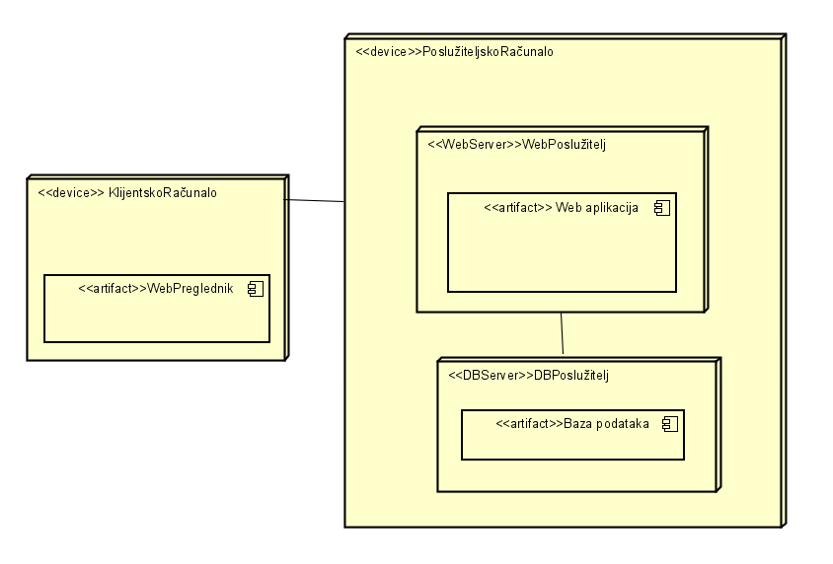
\includegraphics[scale=0.8]{dijagrami/DijagramRazmjestaja}
				\caption{Specifikacijski dijagram razmještaja}
			\end{figure}
			
			\begin{figure}
				\centering
				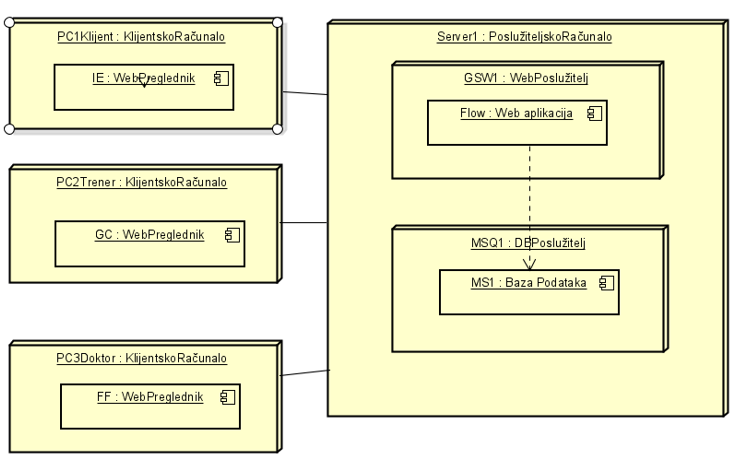
\includegraphics[scale=1]{dijagrami/DijagramRazmjestaja2}
				\caption{Dijagram razmještaja instanci}
			\end{figure}
			\eject 
		
		\section{Upute za puštanje u pogon}
		
			Ove upute su pisane za operacijski sustav Windows 10, aplikaciju je moguće pokrenuti i na drugim operacijskim sustavima, ali treba se voditi računa da se programi drukčije instaliraju na njima i da su naredbe različite.
			\\
			Potrebno je preuzeti installer datoteku s web stranice
			\\ 
			\texttt{\small https://www.postgresql.org/}
			\\
			i provesti standardnu instalaciju PostgreSQL baze podataka na računalo. Bitno je zapamtiti korisničko ime i lozinku koja se postavlja u instalaciji jer će biti potrebne za kasnije spajanje na bazu podataka. Nakon instalacije potrebno je pokrenuti \texttt{\textit{pgAdmin.exe}} koji će otvoriti sučelje za upravljanje bazama podataka.
			
		
			Zatim treba stvoriti novu bazu podataka tako da se na izborniku koji se prikaže desnim klikom na \texttt{\textit{'databases'}} odabere opcija \texttt{\textit{'Create->Database...'}}(ime je proizvoljno).
			
			\begin{figure}[h]
				\centering
				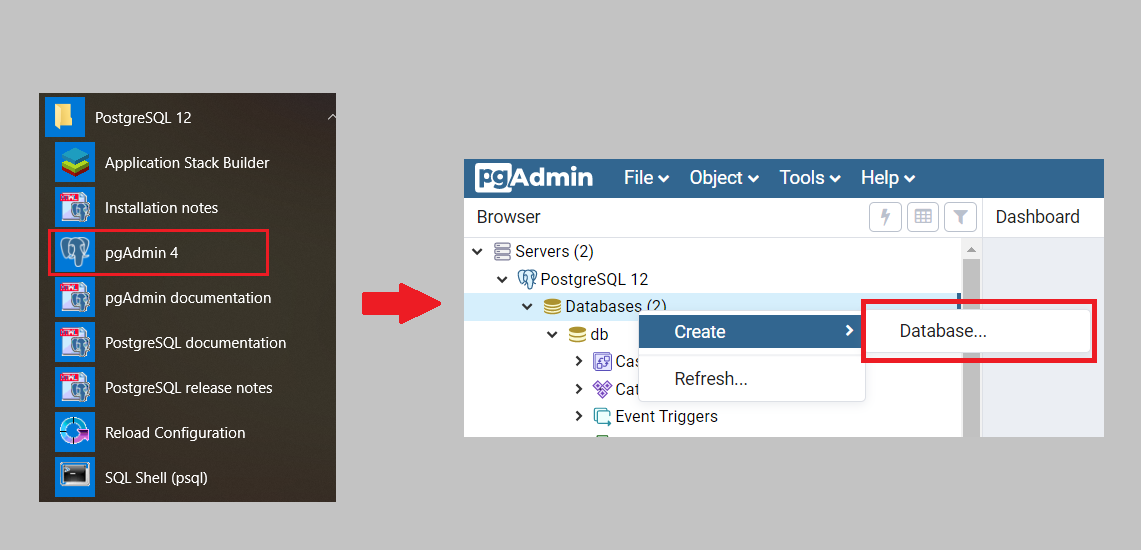
\includegraphics[scale=0.7]{slike/pustanjeupogon/a.png}
				\caption{Stvaranje baze podataka}
			\end{figure}
			
			Backend aplikacije pisan je u programskom jeziku Java, stoga računalo mora na sebi imati instaliran Java Development Kit(JDK) verzija 13. Preuzeti ga je moguće sa službene web stranice:
			\\
			\texttt{\small https://www.oracle.com/technetwork/java/javase/downloads/index.html}
			\\
			Provesti standardnu instalaciju i provjeriti je li sve ispravno instalirano tako da se otvori Command Prompt i upiše \textbf{\texttt{'java --version'}}, ako je sve uredu ispisati će se verzija instalirane jave.
			
			\begin{figure}[h]
				\centering
				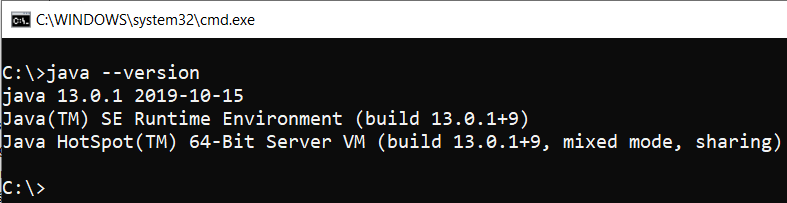
\includegraphics[scale=0.6]{slike/pustanjeupogon/javaversion.png}
				\caption{Provjera je li JDK ispravno instaliran}
			\end{figure}

			U pisanju backenda korišten je Spring framework te zato računalo mora imati instaliran Maven koji vodi računa o svim zavisnostima (dependencies) koje projekt ima. Potrebno je preuzeti zip arhivu s web stranice:
			\\
			\texttt{\small https://maven.apache.org/download.cgi}
			\\
			te ju raspakirati u željeni direktorij. Potom, podesiti environment varijable operacijskog sustava tako da otvorite \texttt{\textit{'System Properties'}} (to je moguće na par načina, ali najlakše je tako da se u polje za pretraživanje upiše: \texttt{\textit{'edit the system en...'}}) i odaberete \texttt{\textit{'Edit the system environment variables'}}.
			
			\begin{figure}[h]
				\centering
				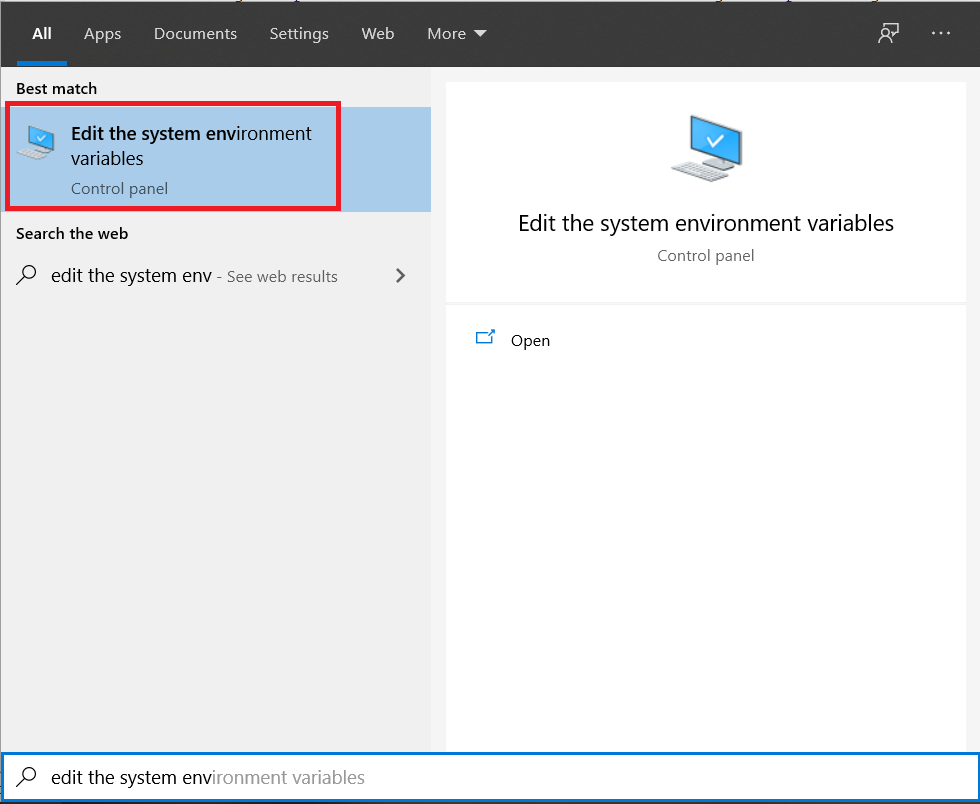
\includegraphics[scale=0.45]{slike/pustanjeupogon/search.png}
				\caption{Otvaranje System Properties}
			\end{figure}
			
			U prozoru koji se otvorio odaberite \texttt{\textit{'Environment Variables'}}, nakon toga odabrati opciju \texttt{\textit{'New'}} u dijelu sučelja \texttt{\textit{'System Variables'}}, u polje \texttt{\textit{'Variable name'}} upisati \texttt{\textit{'MAVEN\_HOME'}}, a u polje \texttt{\textit{'Variable value'}} upisati putanju direktorija koji je nastao raspakiravanjem zip arhive. Potom je potrebno odabrati opciju \texttt{\textit{'Edit'}} za varijablu \texttt{\textit{'Path'}} u polju \texttt{\textit{'System Variables'}} i kada se otvori novi prozor odabrati opciju \texttt{\textit{'New'}} te upisati \texttt{\small '\%MAVEN\_HOME\%\textbackslash bin'}. Maven bi sada trebao biti uspješno instaliran, provjeriti tako da se u Command Prompt upiše naredba \texttt{\textbf{'mvn --version'}}.
			
			\begin{figure}[h]
				\centering
				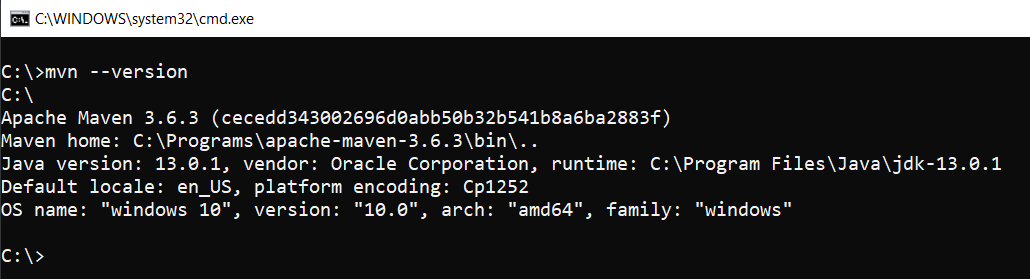
\includegraphics[scale=0.5]{slike/pustanjeupogon/mavenversion.png}
				\caption{Provjera je li Maven ispravno instaliran}
			\end{figure}
		
			Frontend aplikacije napisan je koristeći React Javascript library, stoga računalo mora imati instaliran Node.js kako bi ga mogli pokrenuti. S web stranice: 
			\\
			\texttt{\small https://nodejs.org/en/}
			\\
			preuzeti i pokrenuti installer datoteku. Provesti standardnu instalaciju. Provjeriti je li instalacija uspješna tako da se u Command Prompt upiše naredba \texttt{\textbf{'node --version'}}.
			
			\begin{figure}[h]
				\centering
				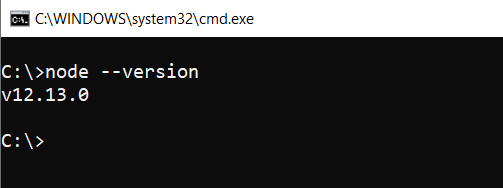
\includegraphics[scale=0.7]{slike/pustanjeupogon/nodeversion.png}
				\caption{Provjera je li Node.js ispravno instaliran}
			\end{figure}
		
			Sada kada su svi potrebni programi instalirani možemo početi s puštanjem aplikacije u pogon. Preuzeti direktorij s GitLab stranice:
			\\
			\texttt{\small https://gitlab.com/fermark/flow}
			\\
			tako da se odabere opcija \texttt{Download->zip}. Raspakirati zip arhivu te navigirati u direktorij \texttt{\small flow\textbackslash src\textbackslash main\textbackslash resources} te otvoriti datoteku \texttt{\textit{ application.properties}}. Potrebno je podesiti nekoliko parametara kako bi se moglo ispravno spojiti na bazu podataka. Za vrijednost parametra \texttt{\small <ime baze podataka>} u polju \texttt{\small spring.datasource.url} potrebno je upisati ime vaše baze podataka. U polja \texttt{\small username} i \texttt{\small password} upisati korisničko ime i lozinku koju ste odabrali kada ste instalirali PostgreSQL bazu podataka. Spremiti izmijene u datoteci.
			
			\begin{figure}[h]
				\centering
				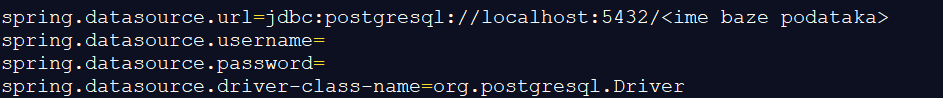
\includegraphics[scale=0.8]{slike/pustanjeupogon/app.png}
				\caption{Izmjena datoteke 'application.properties'}
			\end{figure}
			
			Otvoriti Command Prompt i navigirati u direktorij \texttt{\small \textbackslash flow} te tamo izvršiti naredbu \texttt{\textbf{'mvn install'}}. Time se stvorila izvršna datoteka tipa \texttt{'jar'} u poddirektoriju \texttt{\small target}. Sada je potrebno postaviti i frontend dio aplikacije. U Command Promptu navigirati u direktorij \texttt{\small \textbackslash flow\_front} te tamo izvršiti naredbu \texttt{\textbf{'npm install'}} koja će preuzeti biblioteku React. Potom u istome direktoriju je potrebno izvršiti naredbe \texttt{\textbf{'npm install react-router-dom --save'}} i \texttt{\textbf{'npm install axios --save'}}, a te dvije naredbe će preuzeti potrebne zavisnosti (dependecies) projekta.
			\\
			Sada još jedino preostaje pokrenuti aplikaciju. U direktoriju \texttt{\small \textbackslash flow\_front} izvršiti naredbu \texttt{\textbf{'npm start'}}, frontend dio aplikacije će se pokrenuti. Zatim je potrebno otvoriti novu instancu Command Prompta i u direktoriju \texttt{\small \textbackslash flow\textbackslash target} izvršiti naredbu \texttt{\textbf{'java -jar flow-0.0.1-SNAPSHOT.jar'}}. Ta će naredba pokrenuti backend dio aplikacije koji automatski stvara sve potrebne tablice u bazi podataka, jedino što je još potrebno napraviti je ubaciti u bazu podataka podatke za prijavu administratora. Ponovo pokrenuti sučelje za upravljanje bazom podataka \texttt{\textit{pgAdmin}} i pritisnuti desni klik na vašoj bazi podataka te odabrati opciju \texttt{\textit{Query Tool...}}.
			
			\begin{figure}[h]
				\centering
				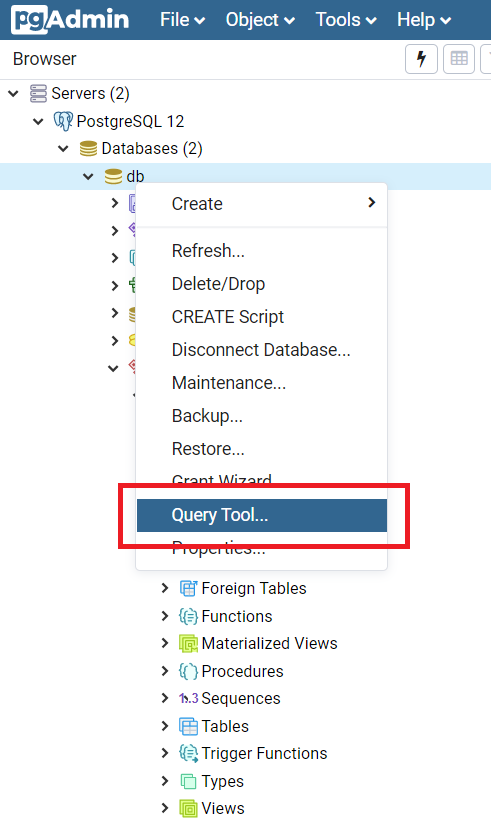
\includegraphics[scale=0.5]{slike/pustanjeupogon/query.png}
				\caption{Otvaranje Query Toola u pgAdmin sučelju}
				
			\end{figure}
			\newpage
			 U polje \texttt{\small Query Editor} upisati naredbu \texttt{\textbf{'INSERT INTO client VALUES ('1', 'ADMIN', 'ADMIN, 'ADMIN, 'ADMIN');'}} i izvršiti ju pritiskom na gumb s ikonom munje.
			
			\begin{figure}[h]
				\centering
				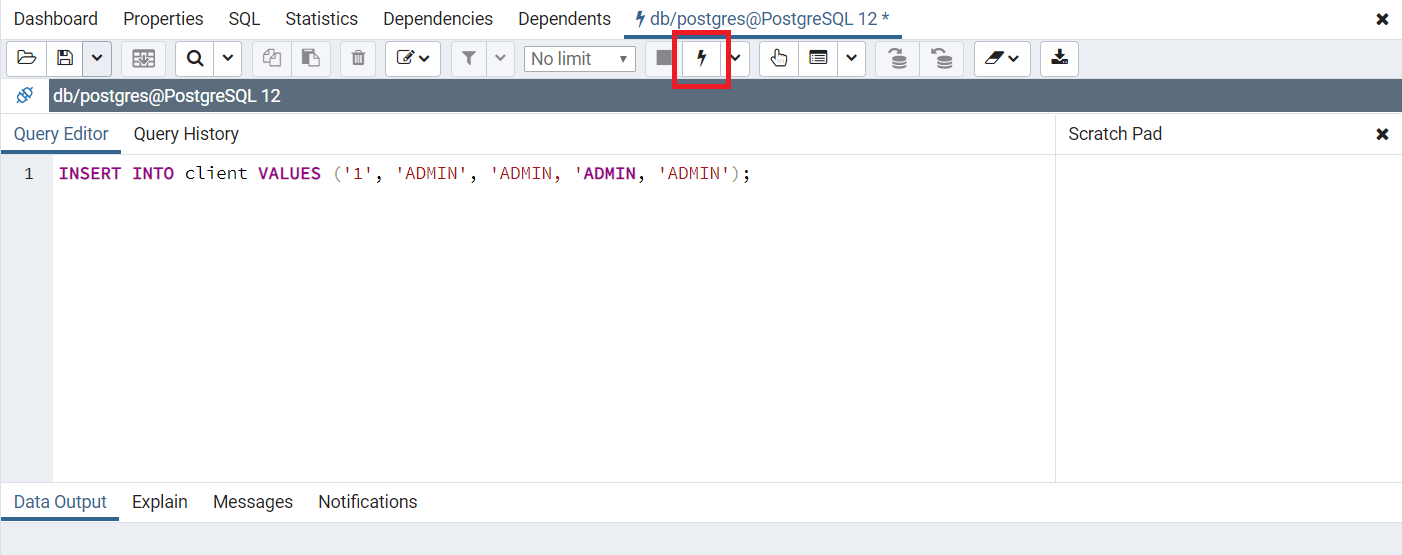
\includegraphics[scale=0.5]{slike/pustanjeupogon/insert.png}
				\caption{Izvršavanje naredbe u sučelju pgAdmin}
			\end{figure}
			
			Aplikacija je pokrenuta i moguće joj je pristupiti na URL
			\\
			\texttt{ \small http://localhost:3000/}
			
			
			\eject 
	\chapter{Zaključak i budući rad}
		
		Nakon što je aplikacija razvijena i postala javno dostupna stavljanjem na server, slijedi razdoblje u kojem bi se trebalo raditi na kontinuiranom poboljšavanju i optimiziranju performansi same aplikacije. To uključuje samo održavanje zdravlja izvorne aplikacije i njezinih funkcionalnosti, kao i proširivanje same aplikacije prema zahtjevima i potrebama njihovih korisnika. Rad na projektu aplikacije ne završava u trenutku njena puštenja u javnost, jer se tek tada treba krenuti u njenu prilagodbu zahtjevima korisnika
		
		\eject 
	\chapter*{Popis literature}
		\addcontentsline{toc}{chapter}{Popis literature}
	 	
 		\textbf{\textit{Kontinuirano osvježavanje}}
	
		\textit{Popisati sve reference i literaturu koja je pomogla pri ostvarivanju projekta.}
		
		
		\begin{enumerate}
			
			
			\item  Oblikovanje programske potpore, FER ZEMRIS, \url{http://www.fer.hr/predmet/opp}
			
			\item  I. Sommerville, "Software engineering", 8th ed, Addison Wesley, 2007.
			
			\item  T.C.Lethbridge, R.Langaniere, "Object-Oriented Software Engineering", 2nd ed. McGraw-Hill, 2005.
			
			\item  I. Marsic, Software engineering book``, Department of Electrical and Computer Engineering, Rutgers University, \url{http://www.ece.rutgers.edu/~marsic/books/SE}
			
			\item  The Unified Modeling Language, \url{https://www.uml-diagrams.org/}
			
			\item  Astah Community, \url{http://astah.net/editions/uml-new}
		\end{enumerate}
		
		 
	
	
	\begingroup
	\renewcommand*\listfigurename{Indeks slika i dijagrama}
	%\renewcommand*\listtablename{Indeks tablica}
	%\let\clearpage\relax
	\listoffigures
	%\vspace{10mm}
	%\listoftables
	\endgroup
	\addcontentsline{toc}{chapter}{Indeks slika i dijagrama}


	
	\eject 
		
	\chapter*{Dodatak: Prikaz aktivnosti grupe}
		\addcontentsline{toc}{chapter}{Dodatak: Prikaz aktivnosti grupe}
		
		\section*{Dnevnik sastajanja}
		
		\textbf{\textit{Kontinuirano osvježavanje}}\\
		
		 \textit{U ovom dijelu potrebno je redovito osvježavati dnevnik sastajanja prema predlošku.}
		
		\begin{packed_enum}
			\item  sastanak
			
			\item[] \begin{packed_item}
				\item Datum: u ovom formatu: \today
				\item Prisustvovali: I.Prezime, I.Prezime
				\item Teme sastanka:
				\begin{packed_item}
					\item  opis prve teme
					\item  opis druge teme
				\end{packed_item}
			\end{packed_item}
			
			\item  sastanak
			\item[] \begin{packed_item}
				\item Datum: u ovom formatu: \today
				\item Prisustvovali: I.Prezime, I.Prezime
				\item Teme sastanka:
				\begin{packed_item}
					\item  opis prve teme
					\item  opis druge teme
				\end{packed_item}
			\end{packed_item}
			
			%
			
		\end{packed_enum}
		
		\eject
		\section*{Tablica aktivnosti}
		
			
			
			 
						
			
			\begin{longtabu} to \textwidth {|X[7, l]|X[1, c]|X[1, c]|X[1, c]|X[1, c]|X[1, c]|X[1, c]|X[1, c]|}
								
				\cline{2-8} \multicolumn{1}{c|}{\textbf{}} &     \multicolumn{1}{c|}{\rotatebox{90}{\textbf{Marko Malkoč }}} & \multicolumn{1}{c|}{\rotatebox{90}{\textbf{Petra Zanetti }}} &	\multicolumn{1}{c|}{\rotatebox{90}{\textbf{Ana Marija Ereš }}} &	\multicolumn{1}{c|}{\rotatebox{90}{\textbf{Jan Juričić }}} &
				\multicolumn{1}{c|}{\rotatebox{90}{\textbf{Petra Omrčen }}} &
				\multicolumn{1}{c|}{\rotatebox{90}{\textbf{Martin Čižmešija }}} &	\multicolumn{1}{c|}{\rotatebox{90}{\textbf{Silvana Bakula }}} \\ \hline 
				\endfirsthead
				
			
				\cline{2-8} \multicolumn{1}{c|}{\textbf{}} &     \multicolumn{1}{c|}{\rotatebox{90}{\textbf{Marko Malkoč }}} & \multicolumn{1}{c|}{\rotatebox{90}{\textbf{Petra Zanetti }}} &	\multicolumn{1}{c|}{\rotatebox{90}{\textbf{Ana Marija Ereš }}} &	\multicolumn{1}{c|}{\rotatebox{90}{\textbf{Jan Juričić }}} &
				\multicolumn{1}{c|}{\rotatebox{90}{\textbf{Petra Omrčen }}} &
				\multicolumn{1}{c|}{\rotatebox{90}{\textbf{Martin Čižmešija }}} &	\multicolumn{1}{c|}{\rotatebox{90}{\textbf{Silvana Bakula }}} \\ \hline 
				\endhead
				
				
				\endfoot
							
				 
				\endlastfoot
				
				Upravljanje projektom 		& x &  &  &  &  &  & \\ \hline
				Opis projektnog zadatka 	&  &  &  &  & x &  & \\ \hline
				
				Funkcionalni zahtjevi       &  &  &  &  &  & x &  \\ \hline
				Opis pojedinih obrazaca 	& x &  &  &  &  &  &  \\ \hline
				Dijagram obrazaca 			&  &  &  &  &  & x &  \\ \hline
				Sekvencijski dijagrami 		&  & x & x &  &  &  &  \\ \hline
				Opis ostalih zahtjeva 		&  &  &  & x &  &  &  \\ \hline

				Arhitektura i dizajn sustava	 &  &  &  & x &  &  &  \\ \hline
				Baza podataka				&  &  &  &  &  &  & x  \\ \hline
				Dijagram razreda 			&  & x & x &  &  &  &   \\ \hline
				Dijagram stanja				&  &  &  &  &  &  &  \\ \hline
				Dijagram aktivnosti 		&  &  &  &  &  &  &  \\ \hline
				Dijagram komponenti			&  &  &  &  &  &  &  \\ \hline
				Korištene tehnologije i alati 		&  &  &  &  &  &  &  \\ \hline
				Ispitivanje programskog rješenja 	&  &  &  &  &  &  &  \\ \hline
				Dijagram razmještaja			&  &  &  &  &  &  &  \\ \hline
				Upute za puštanje u pogon 		&  &  &  &  &  &  &  \\ \hline 
				Dnevnik sastajanja 			&  &  & x &  &  &  &  \\ \hline
				Zaključak i budući rad 		&  &  &  &  &  &  &  \\  \hline
				Popis literature 			&  & x &  &  &  &  &  \\  \hline
				&  &  &  &  &  &  &  \\ \hline \hline
				\textit{front end} 				& x &  &  &  &  & x &  \\ \hline 
				\textit{izrada baze podataka} 		 			&  & x &  &  & x &  & x \\ \hline 
				\textit{spajanje s bazom podataka} 							& x & x & x & x & x &  & x \\ \hline
				\textit{back end} 							&  &  & x & x &  &  &  \\  \hline
				 							
				
				
			\end{longtabu}
					
					
		\eject
		\section*{Dijagrami pregleda promjena}
		
		\textbf{\textit{dio 2. revizije}}\\
		
		\textit{Prenijeti dijagram pregleda promjena nad datotekama projekta. Potrebno je na kraju projekta generirane grafove s gitlaba prenijeti u ovo poglavlje dokumentacije. Dijagrami za vlastiti projekt se mogu preuzeti s gitlab.com stranice, u izborniku Repository, pritiskom na stavku Contributors.}
		
	


\end{document}